\subsection{Borrow Checker}
\label{sec:BorrowCheckerDesign}

The \borrowChecker{} implements the visitor pattern (see
section~\ref{sec:VisitorDesign}) and uses this to traverse the \ast{} in a depth first
left to right pattern. It uses two tables a \texttt{symbolTable} and
\texttt{referenceTable} to keep track of the scope and the
references of each variable.

\begin{figure}[ht]
  \centering
  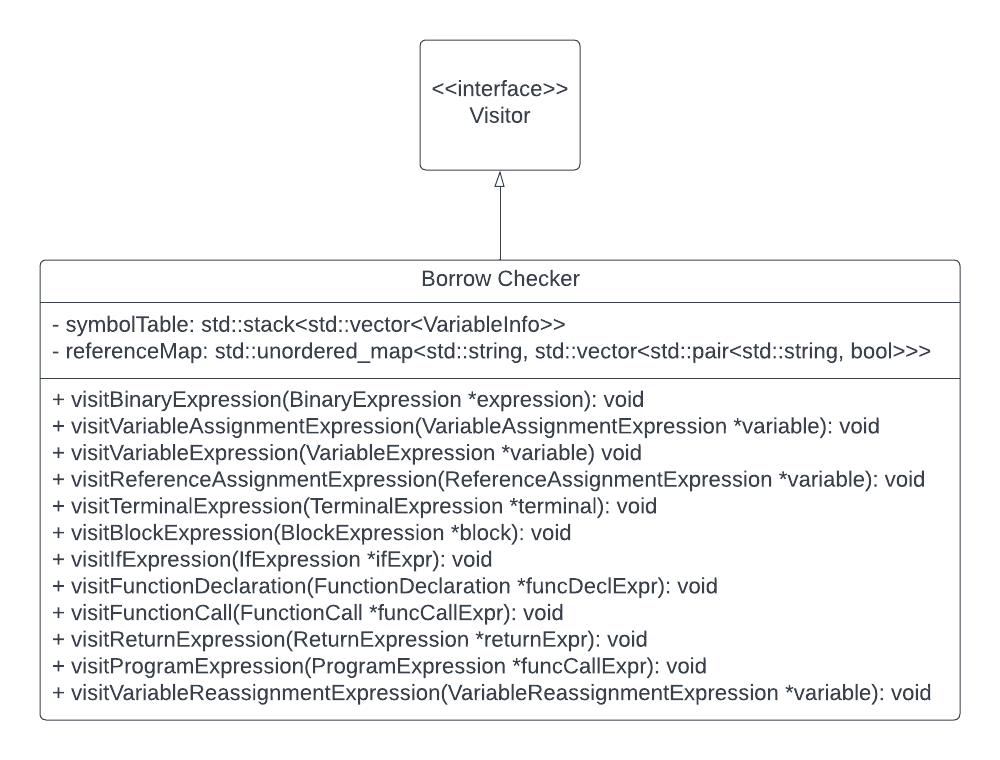
\includegraphics[width=0.8\textwidth]{02-Body/Design/Images/BorrowChecker.png}
  \caption{Class Diagram for the \borrowchecker.}
  \label{fig:borrowcheckerUML}
\end{figure}


